\documentclass[12pt,a4paper,openright,twoside]{book}
\usepackage[utf8]{inputenc}
\usepackage{disi-thesis}
\usepackage{code-lstlistings}
\usepackage{notes}
\usepackage{shortcuts}
\usepackage{acronym}
\usepackage{float}

\school{\unibo}
\programme{Corso di Laurea in Ingegneria e Scienze Informatiche}
\title{Eterogeneità dei sistemi di Aggregate Programming: estensione del sistema ScaFi per l'uso di robot Thymio}
\author{Elvis Perlika}
\date{\today}
\subject{Objective Oriented Programming}
\supervisor{Chiar.mo Prof. Mirko Viroli}
\cosupervisor{Dott. Gianluca Aguzzi}
\session{III}
\academicyear{2023-2024}

% Definition of acronyms
\acrodef{IoT}{Internet of Thing}
\acrodef{vm}[VM]{Virtual Machine}
\acrodef{FP}{Functional Programming}
\acrodef{RT}{Referential Transparency}
\acrodef{AP}{Aggregate Programming}
\acrodef{OOP}{Objective Oriented Programming}
\acrodef{AC}{Aggregate Computing}
\acrodef{TDM}{Thymio Device Manager}

\mainlinespacing{1.241} % line spacing in mainmatter, comment to default (1)

\begin{document}

\frontmatter\frontispiece

\begin{abstract}	
Max 2000 characters, strict.
\end{abstract}

\begin{dedication} % this is optional
    Qualsiasi tecnologia sufficientemente avanzata è indistinguibile dalla magia. \\ Terza Legge di Arthur C. Clarke
\end{dedication}

%----------------------------------------------------------------------------------------
\tableofcontents   
\listoffigures     % (optional) comment if empty
\lstlistoflistings % (optional) comment if empty
%----------------------------------------------------------------------------------------

\mainmatter

%----------------------------------------------------------------------------------------
\chapter{Introduction}
\label{chap:introduction}
%----------------------------------------------------------------------------------------

Write your intro here.
\sidenote{Add sidenotes in this way. They are named after the author of the thesis}

You can use acronyms that your defined previously,
such as \ac{IoT}.
%
If you use acronyms twice,
they will be written in full only once
(indeed, you can mention the \ac{IoT} now without it being fully explained).
%
In some cases, you may need a plural form of the acronym.
%
For instance,
that you are discussing \acp{vm},
you may need both \ac{vm} and \acp{vm}.

\paragraph{Structure of the Thesis}

\note{At the end, describe the structure of the paper}

%----------------------------------------------------------------------------------------
\chapter{Background}
\label{chap:background}
%----------------------------------------------------------------------------------------

% I suggest referencing stuff as follows: \cref{fig:random-image} or \Cref{fig:random-image}

\begin{figure}
    \centering
    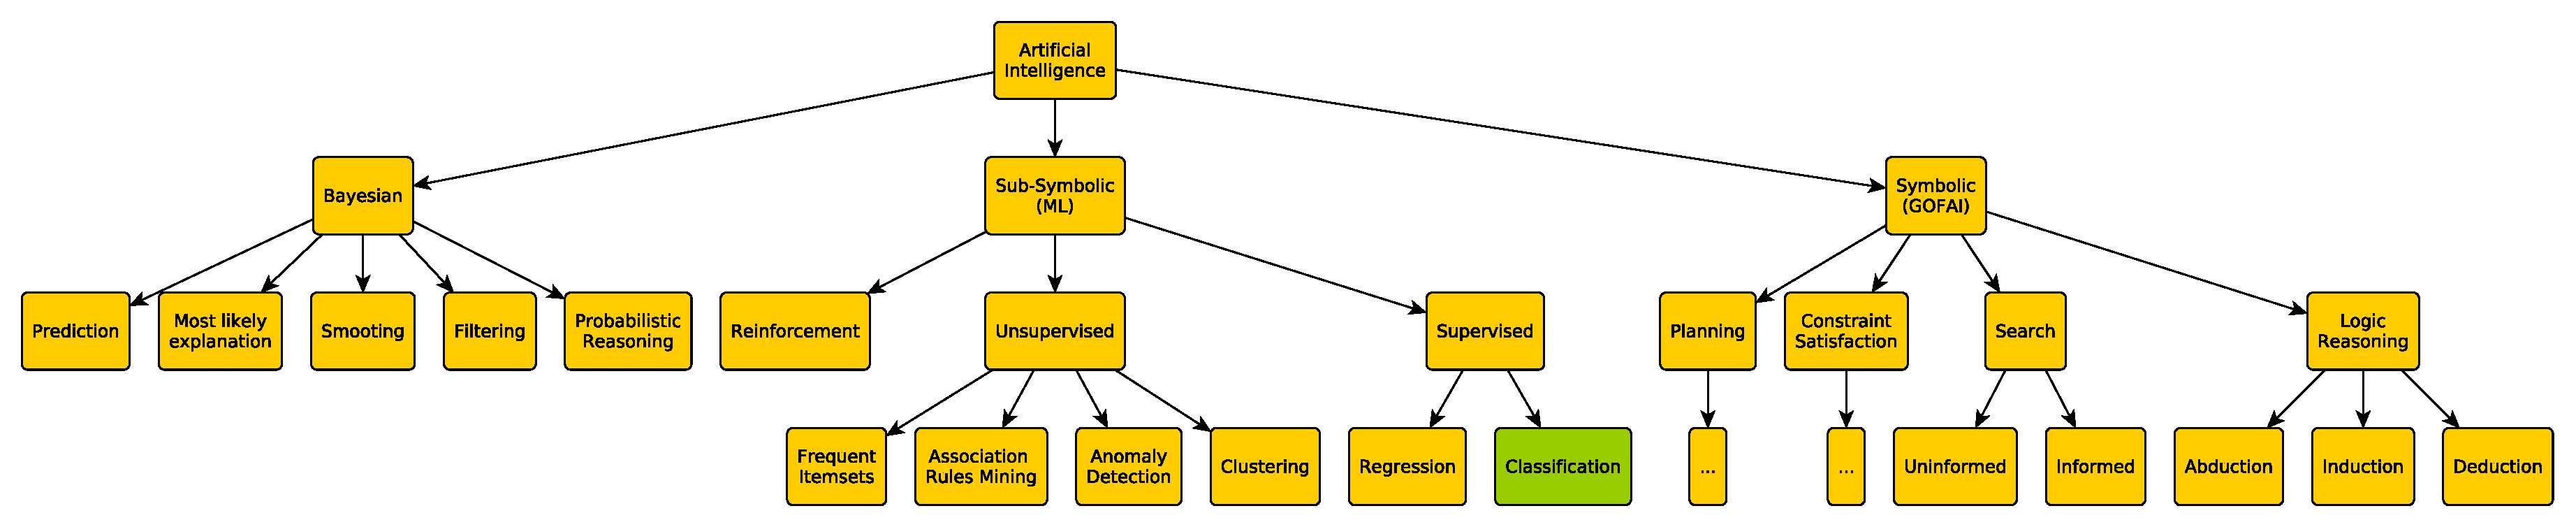
\includegraphics[width=.8\linewidth]{figures/random-image.pdf}
    \caption{Some random image}
    \label{fig:random-image}
\end{figure}

\section{Paradigma OOP e Programmazione Funzionale}

\subsection{Paradigma OOP}

L'Objective Oriented Programming è un paradigma nel senso stretto del termine poiché rappresenta un modo di organizzare e rappresentare un mondo. 
Il paradigma in questione deve la sua potenza nella capacità di simulare entità reali ed è riassumibile con la frase \textit{Everything is an Object}. 
È rilevante parlare di OOP in quanto il paradigma di programmazione funzionale, che è alla base di ScaFi, è un'estensione di esso. 
Il potere della programmazione ad Oggetti (OOP), come detto precedentemente, risiede nella capacità di simulare un mondo e permette di farlo grazie agli "oggetti", essi sono istanze di Classi, le quali a loro volta sono strutture dati astratte che permettono ad ogni loro istanza di avere uno stato (definito dai \textit{fields}) e un comportamento (definito dai \textit{methods}).
I pilastri della programmazione ad oggetti sono l'incapsulamento, l'ereditarietà e il polimorfismo\cref{fig:OOP}.

\begin{figure}
    \centering
    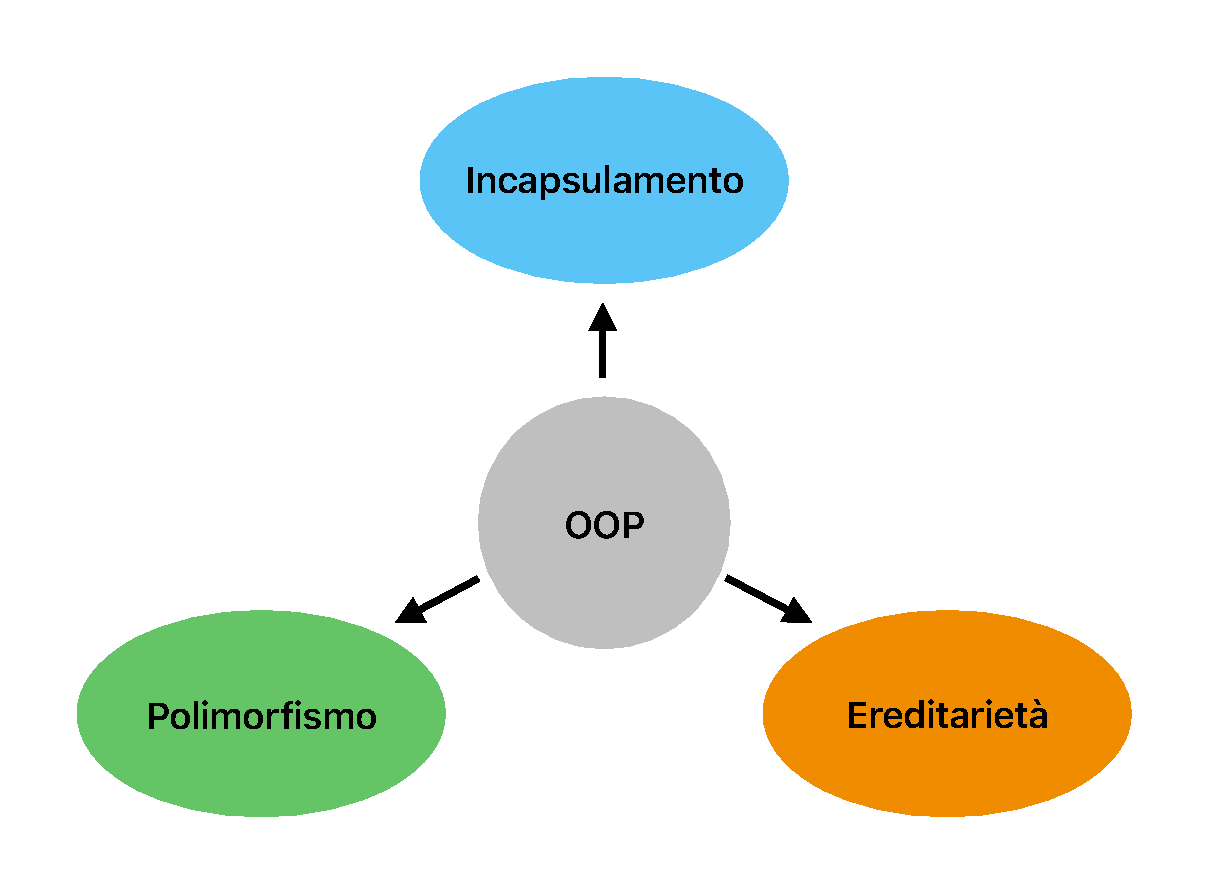
\includegraphics[width=.6\linewidth]{figures/OOP.pdf}
    \caption{Principi della OOP}
    \label{fig:OOP}
\end{figure}

\begin{itemize}
    \item \textbf{Incapsulamento}: Questo principio vuole che i dettagli implementativi di una classe siano nascosti ad altre classi. È un approccio progettuale che mira ad isolare ogni sistema e set di dati. 
    \item \textbf{Ereditarietà}: Con ereditarietà si intende la specializzazione di una classe figlia da una classe madre. Questo permette di creare classi più specifiche che ereditano le proprietà e i metodi della classe madre incoraggiando il riuso del codice.
    \item \textbf{Polimorfismo}: Il polimorfismo è la capacità di un oggetto di assumere più forme. In OOP il polimorfismo è realizzato attraverso l'\textit{overloading} e l'\textit{overriding}. L'overloading è la possibilità di avere più metodi con lo stesso nome ma con diversi parametri \footnote{I parametri possono differire sia in numero che in tipo.}, mentre l'overriding è la possibilità di ridefinire un metodo della classe madre nella classe figlia\footnote{Quando viene chiamato un metodo su un oggetto polimorfico, la scelta di quale implementazione dello stesso metodo scegliere avviene a runtime, in base al tipo effettivo dell'oggetto.}.
\end{itemize}

La programmazione ad oggetti si differenzia dalla più classica programmazione funzionale in quanto controlla la complessità del software supportando la scomposizione gerarchica attraverso sia i dati che l'astrazione procedurale.
Tra i benefici della OOP troviamo la predisposizione al miglioramento della qualità e della leggibilità del codice e la facilità di manutenzione.

Non è, tuttavia, priva di difetti, richiede un particolare impegno gestire il sistema da realizzare all'aumentare della sua complessità. Altri paradigmi, come la programmazione funzionale, possono essere più adatti a determinati problemi.

\subsection{Programmazione Funzionale}
Nel caso della OOP abbiamo riassunto il paradigma con la frase \textit{"Everything is an Object"}, per la programmazione funzionale possiamo riassumerla con \textit{"Everything is a Function"}. Quando si parla di funzioni nel ambito della \ac{FP} si intendo \textbf{funzioni pure} cioè senza effetti collaterali. Per effetti collaterali si intende che la funzione fa altro oltre a restituire un risultato. Un paio di esempi, presi da \texttt{Functional Programming in Scala}, sono:

\begin{itemize}
    \item Modifica di una variabile
    \item Modifica del campo di un oggetto
    \item Leggere da o scrivere su un file
    \item "Disegnare" sullo schermo
\end{itemize}

Si potrebbe pensare che con l'uso della \ac{FP} si possano costruire solo programmi semplice, nella realtà non c'é alcuna limitazione sulla complessità del software da costruire poiché il paradigma della FP esprime un nuovo modo di pensare e scrivere il codice.

Nel dettaglio, per \textbf{funzione pura} si intende una funzione $f:A\to B$, (una funzione che prende un input di tipo $A$ e restituisce un output di tipo $B$) che mette in relazione ogni elemento di $A$ con esattamente un valore di $B$. Qualsiasi altra operazione che non sia utile a calcolare $f(a)=b$ con $a\in A$ e $b\in B$ deve essere intesa come effetto collaterale della funzione e quindi evitata se si vuole creare una funzione pura.

Un esempio di funzione pura, senza effetti collaterali, è la funzione di somma che prende in input due valori e ne restituisce la loro somma \cref{lst:sum-function}. 

\begin{lstlisting}[language=Scala, label={lst:sum-function}, caption={Esempio di funzione pura in Scala}]
    def sum(a: Int, b: Int): Int = a + b
\end{lstlisting}

Un esempio di funzione non pura, con effetti collaterali, è la funzione che prende in input un valore e lo stampa a schermo \cref{lst:print-function}.

\begin{lstlisting}[language=Scala, label={lst:print-function}, caption={Esempio di funzione non pura in Scala}]
    def print(a: Int): Unit = println(a)
\end{lstlisting}

Formalmente si può definire una funzione pura con il concetto di \ac{RT}:

\begin{quote}
    Una funzione $f$ è Referentially Transparent se per ogni contesto $C$ nel quale la funzione viene inserita, essa può essere sostituta dal risultato della stessa funzione $f$ senza condizionare il risultato di $C$.
\end{quote}

È proprio questa proprietà che permette ad un programma progettato con approccio funzionale di essere maggiormente scalabile e mantenibile.

\section{Paradigma dell'Aggregate Programming}

Nei capitoli precedenti si è esaminata l'evoluzione dal paradigma \ac{OOP} a quello \ac{FP}, la quale, ha permesso di gestire in modo più pratico progetti più complessi e semplificandone la manutenibilità. Una ulteriore, più specifica, evoluzione è quella portata dal paradigma dell'\ac{AP}. Quest'ultimo mira a rendere la progettazione, manutenzione e testing nell'ambito del controllo di dispositivi hardware di larga-scala (anche conosciuti come \textbf{collective adaptive systems (CAS)}).

L'\ac{AC} si basa sulla mappatura di un mondo cyber-fisico in un diverso modello logico. Da un punto di vista strutturale possiamo vedere un sistema aggregato come una rete di dispositivi, che corrispondono ai nodi. I nodi sono connessi tra loro secondo una logica di vicinato, che può essere definita in base alla distanza fisica o alla comunicazione. Da un punto di vista comportamentale, invece, ogni nodo interpreta il programma aggregato solo in relazione al proprio contesto locale. Da un punto di vista delle interazioni, i nodi estraggono informazione dal proprio vicinato e propagano le proprie nello stesso contesto. Queste interazioni son ciò che permettono al contesto locale e globale di influenzarsi reciprocamente.

La tecnica dell'\ac{AP} si basa su 3 principi fondamentali per la costruzione di sistemi robusti e resilienti:

\begin{itemize}
    \item I dettagli implementativi dei sistemi hardware che si vuole andare a manipolare devono essere nascosti così da permettere ai programmatori di concentrarsi solo sulla logica di alto livello del sistema, in alcuni casi è possibile che questa astrazione delle specifiche di basso livello sia tale da poter essere pensato come uno spazio continuo, invece di un insieme di dispositivi separati. Per esempio, invece di immaginarci una stanza piena di sensori, la trattiamo come una area unificata definita da un flusso continuo di dati.
    \item Il programma manipola le strutture dati della rete di dispositivi sia in funzione della loro estensione spaziale che di quella temporale. Approccio particolare utile in sistemi in cui l'informazione cambia in base al luogo.
    \item Ogni dispositivo della rete esegue le operazioni necessarie in autonomia, coordinandosi con i dispositivi vicini attraverso meccanismi robusti e resilienti. In questo modo il sistema rimane fluido ed efficiente anche in situazioni anomale, ad esempio causate dal guasto di un qualche dispositivo.
\end{itemize}

% //TODO: questa parte è terribile, va riscritta-----------------
L'approccio \ac{AP} nella progettazione di sistemi si allontana dal più classico approccio "dispositivo centrico", nel quale ogni dispositivo della rete ha il compito di compiere tutte le operazioni richieste per il raggiungimento della soluzione e simultaneamente comunicare con gli altri dispositivi della rete. Questo approccio, seppur semplice, è poco scalabile e difficile da mantenere al crescere della complessità del sistema. Il nuovo paradigma prevede la scomposizione in componenti del programma assegnato ad ogni dispositivo, ogni componente esegue un compito specifico e comunica principalmente solo con i componenti dello stesso tipo presenti nel suo intorno per eseguire un servizio ed eventualmente con un altro componente presente nello stesso dispositivo al fine di realizzare una nuova soluzione inerente ad un'altro servizio. 
% -----------------------------------------------------------

Il paradigma \ac{AP}, che ha permesso la creazione di framework come Protelis e ScaFi, si basa sul concetto dei \textit{campi di calcolo}. Per \textit{campi di calcolo} o \textit{computationals fields} si intende la mappatura degli elementi del dominio in cui si opera in un insieme di valori.
I campi di calcolo vengono utilizzati per standardizzare le interazioni tra i dispositivi, permettendo di analizzare e progettare sistemi distribuiti in modo più semplice e intuitivo. L'idea di campo prende ispirazione dai campi fisici, ad esempio quello magnetico. Ogni dispositivo della rete è considerato come un punto nello spazio ed il campo rappresenta un dato valore assegnato ad ognuno di questi punti. Questo insieme di valori, che chiameremo \textit{campi} o \textit{fields} rappresentano lo stato del sistema in un dato istante.

Ogni dispositivo del proprio sistema aggregato esegue una computazione in modo asincrono attraverso i \textbf{sense-compute-(inter)act rounds}, ogni round è composto da tre fasi concettuali:

\begin{enumerate}
    \item \textbf{Aggiornamento del contesto}: ogni nodo memorizza il suo stato precedente, i dati ambientali restituiti da eventuali sensori e le informazioni ricevute dai nodi vicini.
    \item \textbf{Esecuzione del Programma Aggregato}: il campo di ogni nodo viene computato in base al contesto locale e produce un valore di output.
    \item \textbf{Azione}: in questa fase il nodo può effettuare una o entrambe le seguenti azioni:
    \begin{enumerate}
        \item \textbf{Condivisione}: il nodo condivide il proprio export verso i nodi del suo vicinato
        \item \textbf{Controllo di attuatori}: l'output del nodo viene utilizzato per l'esecuzione di uno o più attuatori nel proprio ambiente
    \end{enumerate}
\end{enumerate}

Posizionandoci in un livello più implementativo troviamo i seguenti costrutti per la manipolazione dei campi: 
% //TODO: citare il paper "Aggregate Programming for the Internet of Things" per i seguenti costrutti

\begin{itemize}
    \item \textbf{Functions}: funzioni $$ b(e_1,\dots,e_n) $$ applicate agli argomenti $e_1,\dots,e_n$. Possono essere sia funzioni matematiche, logiche o algoritmiche ma possono anche rappresentare sensori o attuatori.
    \item \textbf{Dynamics}: $$ rep(x \leftarrow v){s_1;\dots;s_n} $$ rappresenta un una variabile di stato locale $x$, inizialmente inizializzata con il valore $v$ e che può essere modificata dalle istruzioni $s_1,\dots,s_n$. In questo modo si definisce un campo dinamico.
    \item \textbf{Interaction}: $$ nbr(s) $$ rappresenta il vicinato di un dispositivo, ovvero l'insieme dei dispositivi con cui è possibile interagire.
    \item \textbf{Restrictions}: $$
        \begin{array}{l}
        \text{if } e \\
        \qquad s_1; \quad \dots \quad s_n; \\
        \text{else} \\
        \qquad s_1'; \quad \dots \quad s_m';
        \end{array}
    $$
    permette di andare a definire sotto spazio del campo principiale in base ad una condizione $e$ sul quale poi andare ad eseguire certe istruzioni invece di altre. È importante che le istruzioni riferite ad un certo sotto spazio non abbiano effetti su altri sotto spazi.
\end{itemize}

\begin{quote}
    \centering
    Come viene eseguito un modello di \ac{AP}?
\end{quote}

Questo paradigma, proprio come quelli precedenti, non è privo di difetti. 
Implementazioni di questo tipo sono difficili da integrare in sistemi programmati in modo più tradizionale, inoltre, dal punto di vista della programmazione sono mancanti i meccanismi per la gestione della concorrenza e della computazione dinamica dei campi. Il framework ScaFi, che vedremo nel prossimo capitolo, cerca di risolvere questi problemi.

% //TODO: capitolo incompleto

\section{ScaFi e Macro-Swarm}

ScaFi è un toolkit open-source basato su Scala per l'\ac{AC} per la progettazione ad alto livello di sistemi aggregati.
Il termine ScaFi deriva dalla unione di Scala e Fields. Scala è un linguaggio java-like moderno e flessibile progettato per unificare il paradigma \ac{OOP} e quello \ac{FP}. È stato progettato per essere coinciso e facilmente leggibile, inoltre si basa sulla Java Virtual Machine, la quale permette l'utilizzo delle librerie Java. L'utilizzo della JVM e la flessibilità del linguaggio sono state le caratteristiche chiave per il raggiungimento della popolarità di questo linguaggio. Il termine Field invece deriva dai \textit{field calculus} (campi di calcolo) di cui abbiamo parlato nei capitoli precedenti.

\subsection{Architettura di ScaFi}

L'Architettura di ScaFi è riassumibile nella immagine \cref{fig:scafi-arc}.

\begin{figure}
    \centering
    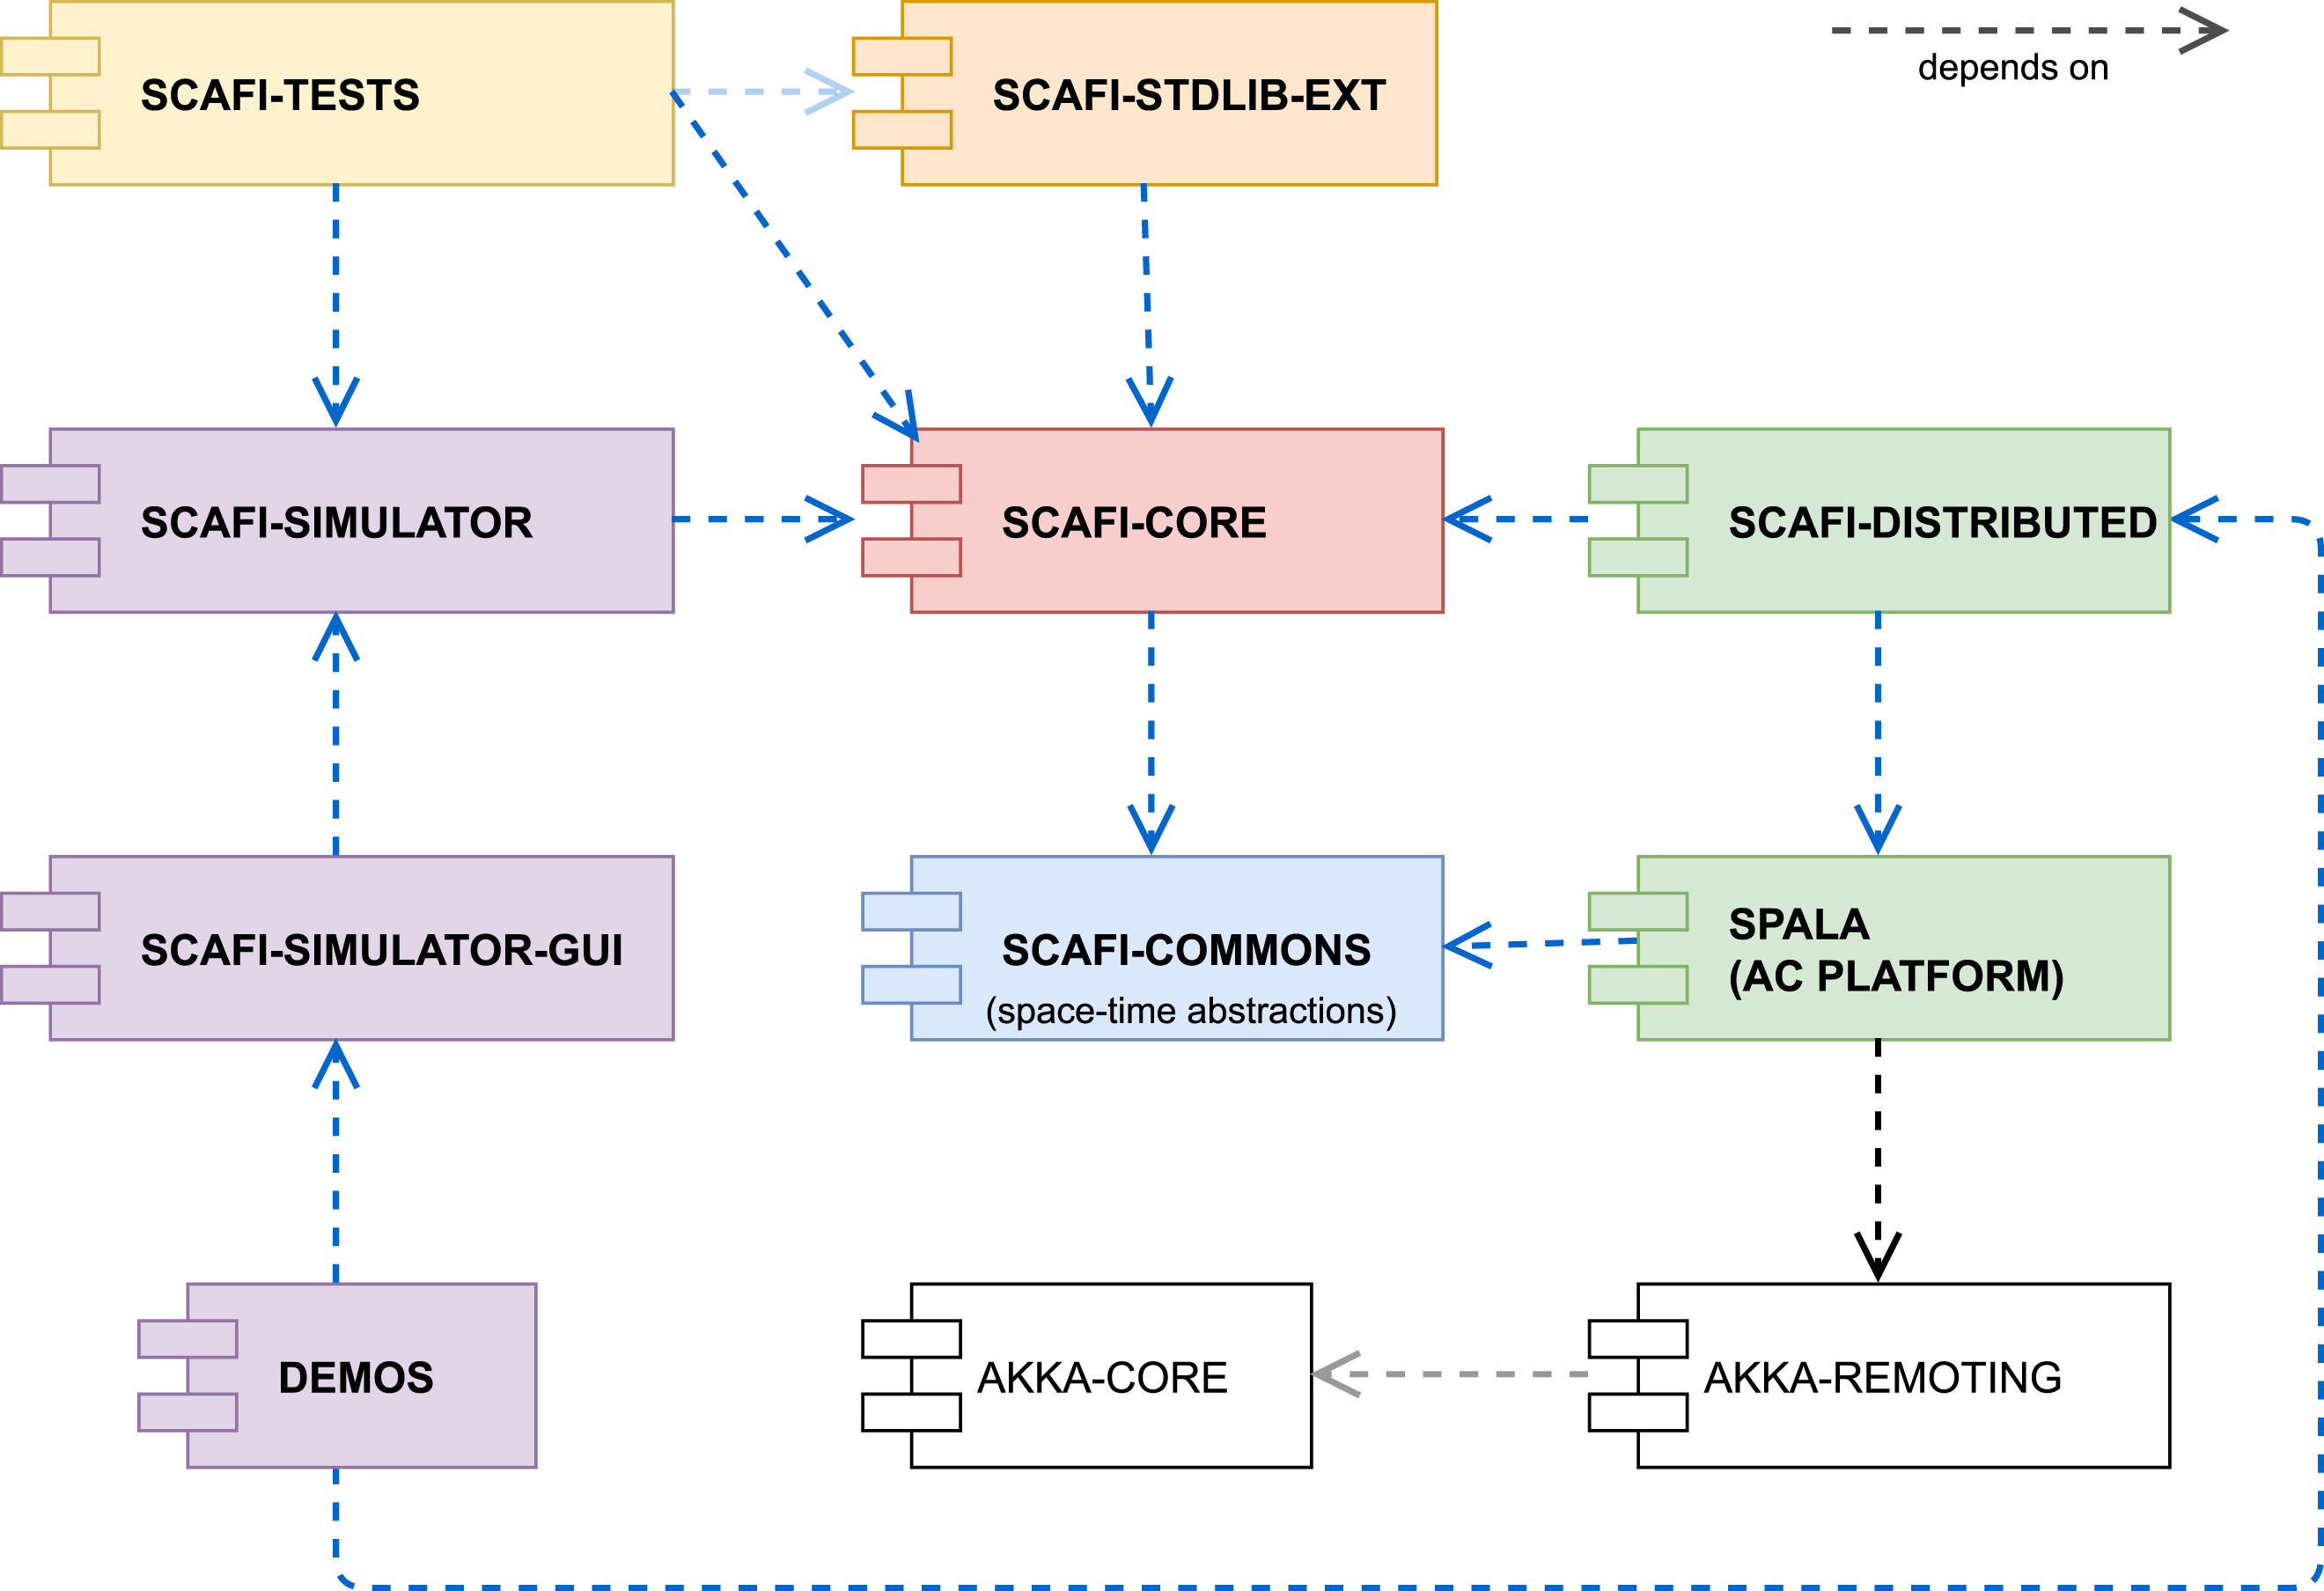
\includegraphics[width=.8\linewidth]{figures/scafi-arc.jpg}
    \caption{Architettura del framework ScaFi}
    \label{fig:scafi-arc}
\end{figure}

Ispezionando la figura, troviamo:

\begin{itemize}
    \item \textbf{scafi-commons}: fornisce le entità di base, ad esempio astrazioni temporali e spaziali
    \item \textbf{scafi-core}: rappresenta il core del framework fornendo il DSL\footnote{Domain Specific Language: linguaggio di programmazione progettato specificamente per risolvere problemi o esprimere concetti di un dominio ristretto. Il DSL di ScaFi (libreria di programmazione) è quindi un linguaggio specifico per creare e valutare programmi di tipo aggregato, utilizzando una sintassi e una semantica pensate appositamente per questo tipo di calcoli e simulazioni.} per la progettazione di sistemi aggregati; con il supporto di librerie standard.
    \item \textbf{scafi-stdlib-ext}: librerie extra
    \item \textbf{scafi-simulator}: fornisce un supporto per la simulazione dei sistemi di \ac{AP} sviluppati
    \item \textbf{scafi-simulator-GUI}: fornisce un'interfaccia grafica per la simulazione
    \item \textbf{spala}: ("spatial scala") si tratta di un \textit{middleware} che permette di eseguire programmi \ac{AC} basati sugli attori ed è indipendente dal DSL di ScaFi
    \item \textbf{scafi-distributed}: layer integrativo per l'utilizzo di \textbf{spala} in ScaFi
\end{itemize}

\begin{quote}
    \centering
    Perché usare Scala?
\end{quote}

Il motivo per cui Scala è un linguaggio particolarmente adatto per la programmazione di sistemi di \ac{AC} è dovuto proprio alla sua flessibilità, essa permette di lavorare sui campi di calcolo, che necessitano di essere supportati dalle seguenti proprietà, in modo molto naturale:

\begin{itemize}
    \item una sintassi coincisa per definire funzioni sui campi, le quali in Scala sono le espressioni standard
    \item meccanismi di controllo sul \textit{quando} e \textit{come} le espressioni vengono valutate
    \item capacità di calcolare lo stato di un campo basandosi sulle informazioni più recenti dei nodi presenti nel suo intorno
\end{itemize}

In Scala ogni valore è un oggetto ed i comportamenti vengono definiti attraverso i metodi. Per implementare un campo di calcolo in Scala andremo a definire gli operato dei campi attraverso la definizione di metodi che verranno interpretati dagli oggetti sui quali sono stati chiamati. Gli oggetti, in questo modo, possono essere visti come macchine virtuali in locale per l'esecuzione degli operatori di campo.

Di seguito l'interfaccia fondamentale per la definizione di un campo di calcolo in Scala (\cref{lst:constructs-scala}):

\lstinputlisting[float=tb,language=Scala,label={lst:constructs-scala},caption={Interfaccia per la definizione di un campo di calcolo in Scala}]{listings/Constructs.scala}

Gli elementi principali di questa interfaccia sono:
\begin{itemize}
    \item \verb|rep(init)(f)| cattura l'evoluzione di stato di un valore inizializzato ad \verb|init| e aggiornato ad ogni round con la funzione \verb|f|
    \item \verb|nbr(expr)|: rileva le comunicazioni relative al valore computato dalla espressione \verb|expr| dei nodi vicini
    \item \verb|foldhood(init)(acc)(expr)|: si occupa, partendo da un valore iniziale \verb|init|, di accumulare i valori computati dai nodi vicini attraverso la funzione di accumulazione \verb|acc| e settare i valori computati dalla espressione \verb|expr| verso i propri vicini
    \item \verb|branch(cond)(th)(el)|: cattura una partizione (spazio-temporale) del dominio in base alla condizione \verb|cond|, se questa è rispettata esegue l'espressione \verb|th| altrimenti \verb|el|
    \item \verb|mid|: provvede ad identificare un certo nodo
    \item \verb|sense(sensorName)|: permette di accedere (ad alto livello) al sensore locale \verb|sensorName|
    \item \verb|nbrvar(sensorName)|: permette di accedere (ad alto livello) ai sensori dei nodi vicini, simile ad \verb|nbr| ma valido per sensori forniti dalla piattaforma, questi sensori forniscono un valore per ciascun vicino
\end{itemize}

In ScaFi, i campi non sono reificati esplicitamente ma esistono solo a livello semantico, questo significa che un'espressione Scala non viene gestita come un'espressione di campo finché non viene passata all'interprete ScaFi.
% //TODO: citare la tesi PhD di Casadei


\section{Thymio e tdmclient}

\begin{quote}
    Thymio è un robot educativo open-source progettato da ricercatori dell'EPFL (Politecnico federale di Losanna), in collaborazione con l'ECAL (Università d'arte e design di Losanna), e prodotto da Mobsya, un'associazione no-profit la cui missione è quella di offrire percorsi STEAM completi e coinvolgenti a studenti di tutte le età.
\end{quote}

Thymio è un robot programmabile con un'ampia varietà di sensori e attuatori, tra cui:
\begin{itemize}
    \item 9 sensori a infrarossi (portata circa 10 cm)
    \item 5 pulsanti a sfioramento (tecnologia capacitiva)
    \item 1 accelerometro a tre assi
    \item 1 termometro
    \item 1 microfono
    \item 1 ricevitore a infrarossi per il telecomando
    \item 39 LED controllabili
    \item 2 motori DC collegati alle ruote
    \item 1 altoparlante
\end{itemize}


Questo dispositivo è stato scelto per essere implementato nella demo per la notte dei ricercatori in quanto è un robot molto versatile e adatto a molteplici applicazioni. Inoltre, il robot è molto diffuso nelle scuole e nei laboratori di robotica educativa, quindi è un'ottima scelta per mostrare il potenziale di ScaFi in un contesto educativo.

Questo piccolo robot nasce per essere programmato con linguaggi a blocchi come VPL, VPL3, Scratch, Blocky e non come Aseba, Python e Ros, tutti accessibili dalla suite dedicata \textit{"Thymio Suite"}.
% //TODO: citare doc a tutti i linguaggi supportati dalla bibliografia
Noi ci concentreremo nel uso di Python. 

% //TODO: da scrivere meglio
Python a differenza di altri linguaggi (ad esempio C/C++) è interpretato e non compilato. I linguaggi compilati prevedono la conversione del programma scritto in un linguaggio ad alto livello in linguaggio macchina per poi farlo eseguire dal processore, occorre quindi compilare il sorgente ad ogni nuova modifica per poi re-eseguirlo. Python, invece, è un linguaggio interpretato, il codice sorgente viene eseguito direttamente dal programma interprete, il quale esegue ogni comando riga per riga.

\begin{figure}
    \centering
    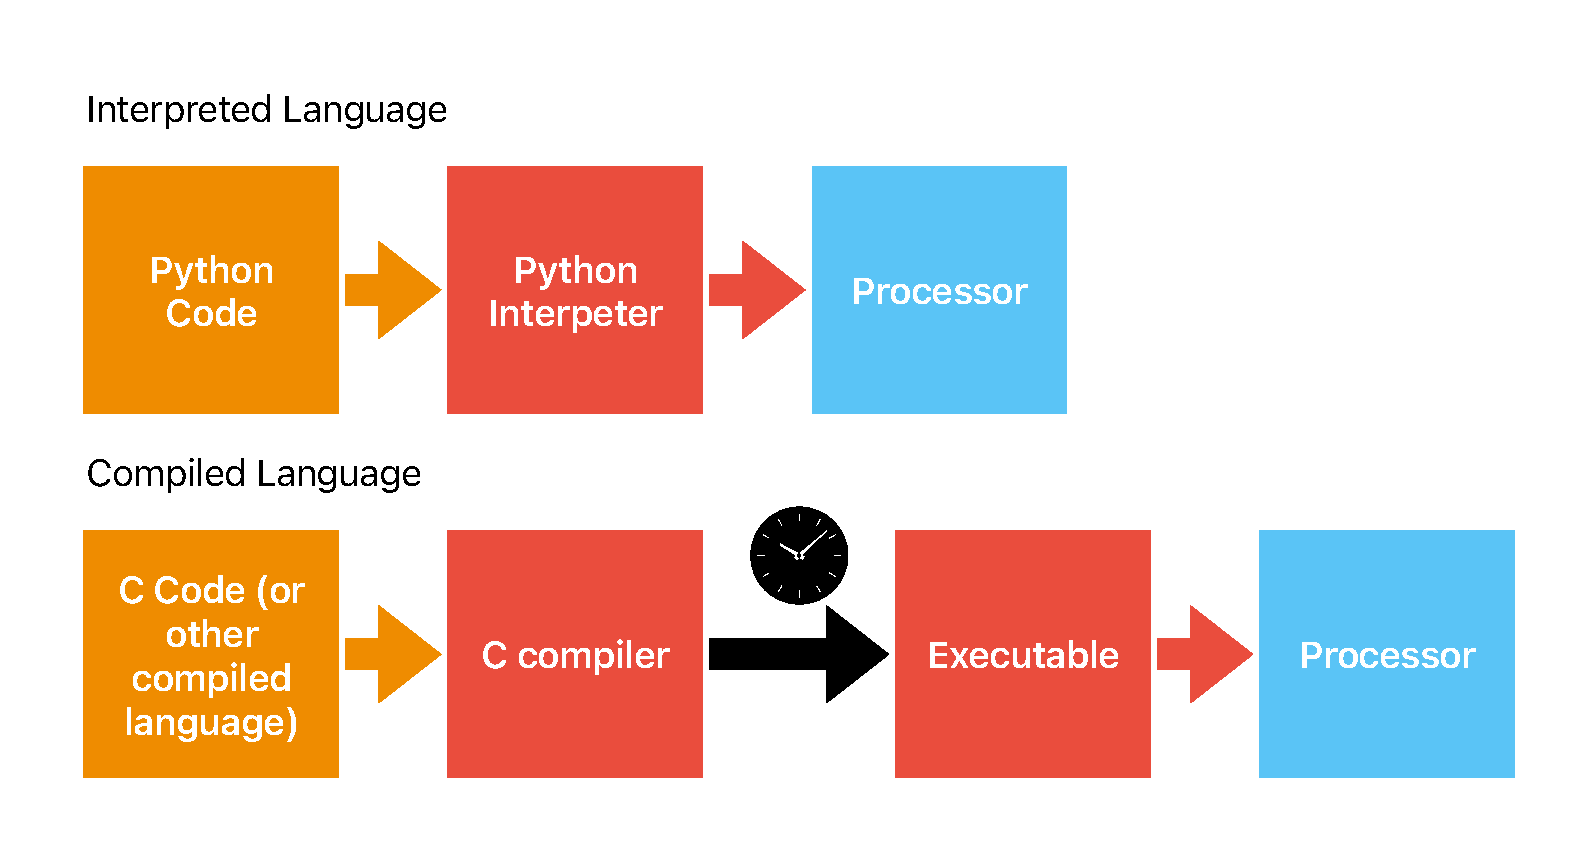
\includegraphics[width=.8\linewidth]{figures/interpreter-compiler.pdf}
    \caption{Interprete vs Compilatore}
    \label{fig:thymio}
\end{figure}

Nel caso del robot Thymio, non è presente un interprete nel suo microcontrollore. È presente, invece, una Aseba Virtual Machine che permette di eseguire programmi scritti in linguaggio Aseba. 

Aseba è un linguaggio di programmazione ad alto livello basato su architettura ad eventi, il che significa che gli eventi sono eseguiti in modo asincrono. Gli eventi sono identificati da un Identificativo ed opzionalmente da un \textit{payload} (dati aggiuntivi). 
Gli eventi possono essere di due tipi:
\begin{itemize}
    \item \textbf{global events}: eventi generati dai nodi e condivisi con la rete
    \item \textbf{local events}: eventi generati da un nodo e non condivisi con la rete (ad esempio un evento generato da un sensore dello stesso nodo)
\end{itemize}

Un esempio di codice Aseba è il seguente \cref{lst:aseba-code}.
% Non è disponibile Aseba quindi useremo Scala
\begin{lstlisting}[language=C, label={lst:aseba-code}, caption={Esempio di codice Aseba con eventi}]
    var state

    callsub init  # Inizializza il programma

    sub init
        state = 0
        call leds.bottom.left(0,0,32)
        call leds.bottom.right(0,32,0)
        call leds.top(32,0,0)

    # Re-inizia quando il pulsante centrale viene premuto
    onevent button.center
        callsub init
\end{lstlisting}

Il \textbf{Thymio Device Manager}, servizio presente nella Thymio Suite, si occupa di tradurre i sorgenti in linguaggio Aseba in Aseba bytecode per poi caricarlo nel robot. Per l'utilizzo di python, invece, è necessario l'utilizzo del modulo \textbf{tdmclient} che si occupa di fare comunicare Python con il \ac{TDM} \cref{fig:tdmclient}. È necessario che la Thymio Suite sia in esecuzione per poter utilizzare il modulo \textbf{tdmclient} il quale necessita a sua volta l'utilizzo di \textbf{Python 3} come interprete.

Questo modulo permette di:
\begin{itemize}
    \item accedere alle variabili, sensori, attuatori del robot
    \item convertire uno script Python in un script Aseba 
    \item inviare codice Aseba al \ac{TDM} che a sua volta invia il relativo bytecode al  robot Thymio 
\end{itemize}

% //TODO: approfondire cosa è Aseba

\begin{figure}
    \centering
    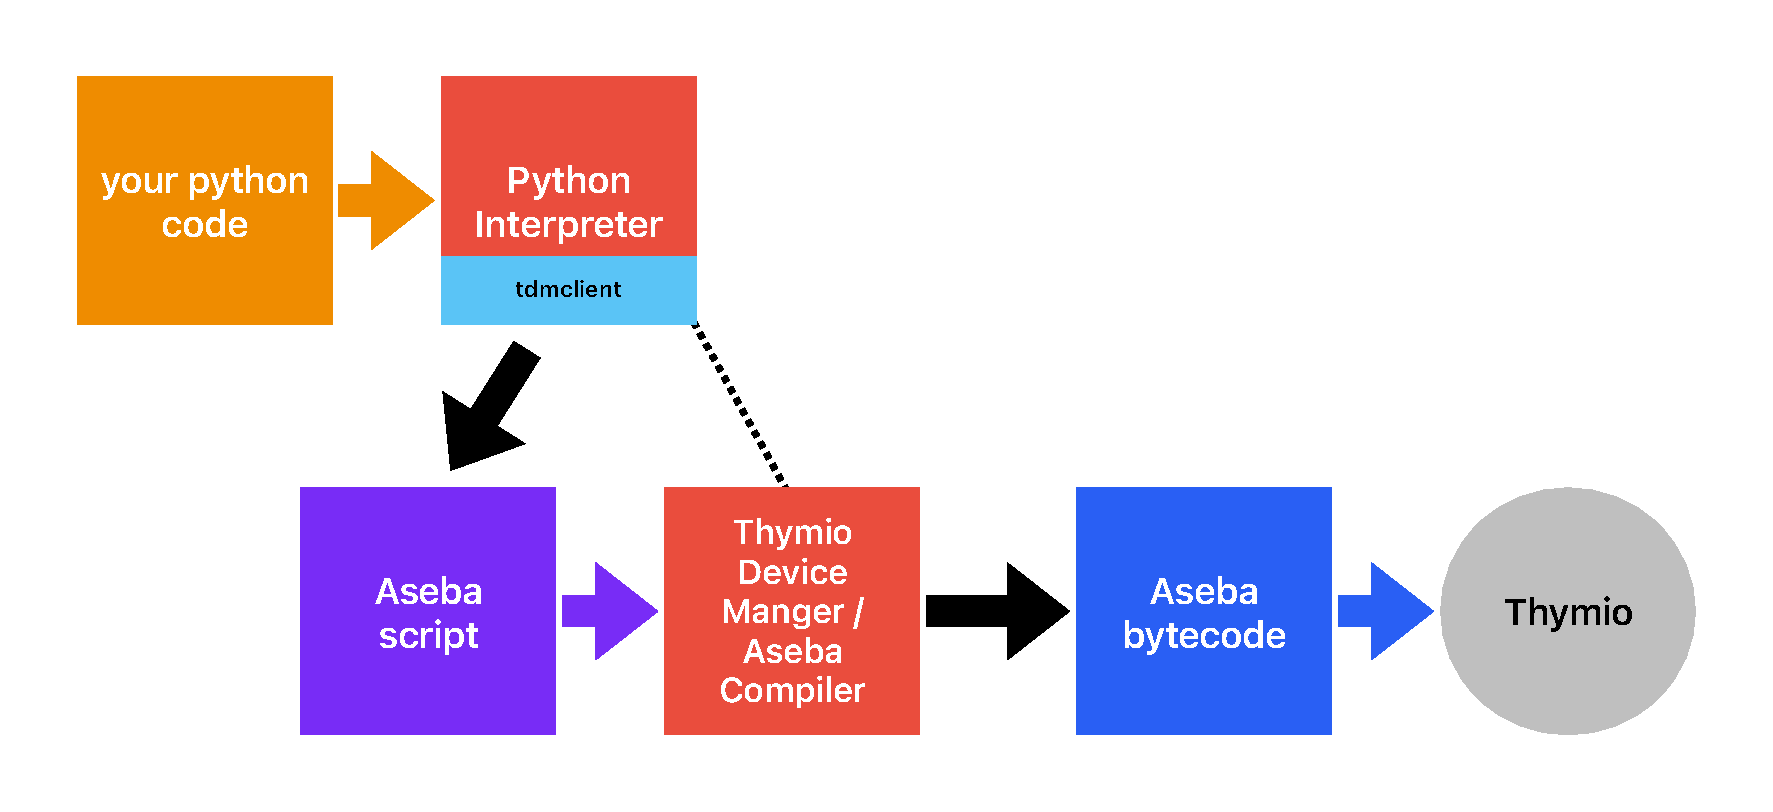
\includegraphics[width=.8\linewidth]{figures/TDM.pdf}
    \caption{Tdmclient workflow}
    \label{fig:tdmclient}
\end{figure}



\section{Aruco Tag}

%----------------------------------------------------------------------------------------
\chapter{Analisi}
\label{chap:analisi}
%----------------------------------------------------------------------------------------

\section{Estensibilità del sistema ad un nuovo modello di Robot (Thymio)}

\section{Gestione dei vincoli di compatibilità del sistema Thymio}


%----------------------------------------------------------------------------------------
\chapter{Design}
\label{chap:design}
%----------------------------------------------------------------------------------------

\section{Architettura server Flask}

\section{File di configurazione}

%----------------------------------------------------------------------------------------
\chapter{Implementazione}
\label{chap:implementazione}
%----------------------------------------------------------------------------------------

\section{Implementazione del server Flask}

\section{Esempi di Algoritmi AP applicati ai Robot Wave e Thymio nello stesso ambiente}

You may also put some code snippet (which is NOT float by default), eg: \cref{lst:random-code}.

\lstinputlisting[float,language=Java,label={lst:random-code}]{listings/HelloWorld.java}

\section{Fancy formulas here}

%----------------------------------------------------------------------------------------
\chapter{Conclusione}
\label{chap:conclusione}
%----------------------------------------------------------------------------------------

%----------------------------------------------------------------------------------------
% BIBLIOGRAPHY
%----------------------------------------------------------------------------------------

\backmatter

\nocite{*} % Remove this as soon as you have the first citation

\bibliographystyle{alpha}
\bibliography{bibliography}

\begin{acknowledgements} % this is optional
Optional. Max 1 page.
\end{acknowledgements}

\end{document}
